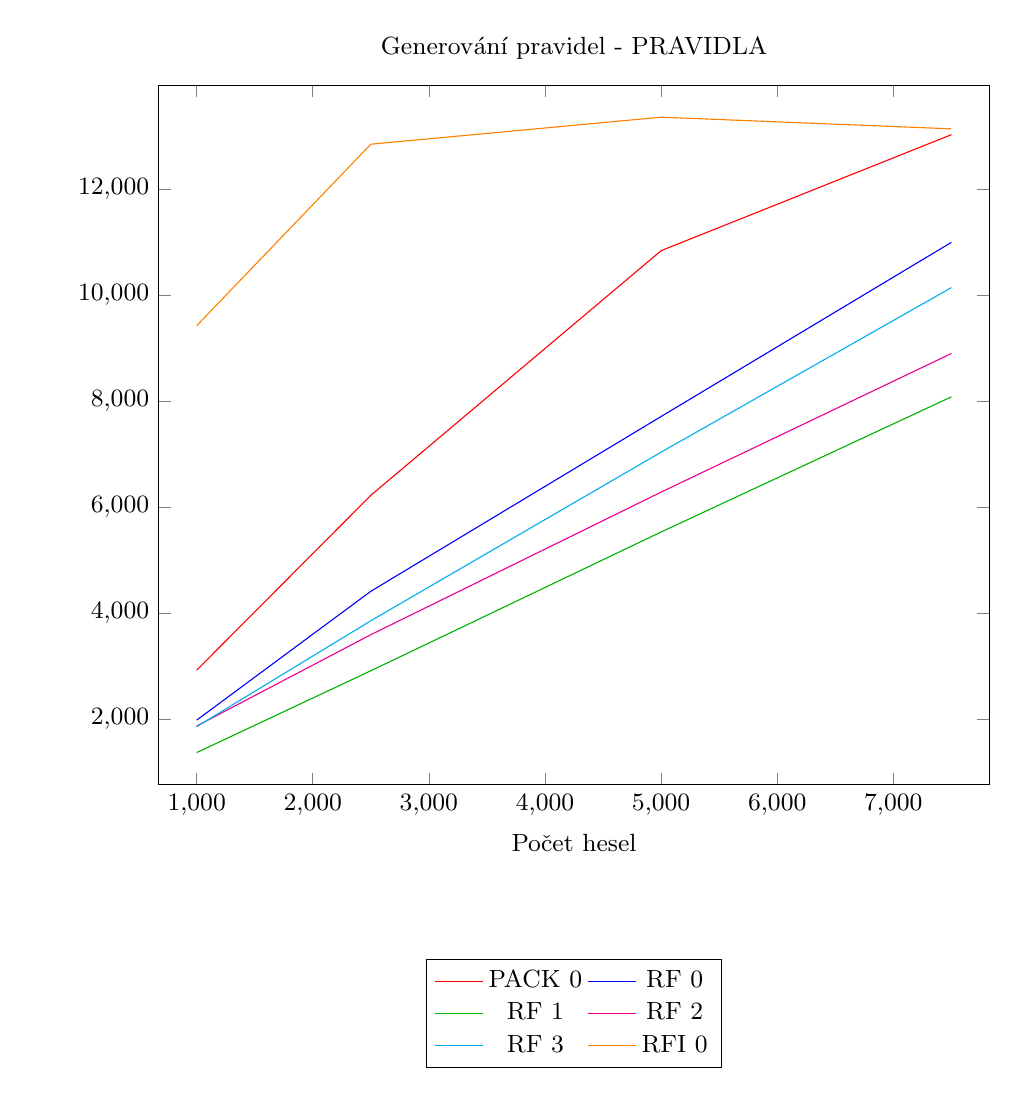
\begin{tikzpicture}
  \begin{axis}[
    width=\linewidth, 
    every axis/.append style={font=\small},
    title={Generování pravidel - PRAVIDLA},
    xlabel={Počet hesel},
    ylabel={\phantom{Počet pravidel}},
    legend style={
      at={(0.5,-0.25)},
      anchor=north,
      legend columns=2,
    },
    enlargelimits=0.05,
    scaled y ticks = false,
    scaled x ticks = false,
    cycle list={
     {red},
     {blue},
     {green!70!black},
     {magenta},
     {cyan},
     {orange},
     {violet},
     {purple},
     {gray},
     {darkgray}%
    }
    ]
    
    \addplot coordinates {
      (1000, 2921.0) 
      (2500, 6221.0) 
      (5000, 10837.0) 
      (7500, 13026.0) 
      }; % PACK 0
    
    \addplot coordinates {
      (1000, 1978.0) 
      (2500, 4410.0) 
      (5000, 7708.0) 
      (7500, 10994.0) 
      }; % RF 0
    
    \addplot coordinates {
      (1000, 1366.0) 
      (2500, 2910.0) 
      (5000, 5529.0) 
      (7500, 8079.0) 
      }; % RF 1
    
    \addplot coordinates {
      (1000, 1867.0) 
      (2500, 3591.0) 
      (5000, 6281.0) 
      (7500, 8897.0) 
      }; % RF 2
    
    \addplot coordinates {
      (1000, 1855.0) 
      (2500, 3854.0) 
      (5000, 7035.0) 
      (7500, 10140.0) 
      }; % RF 3
    
    \addplot coordinates {
      (1000, 9421.0) 
      (2500, 12846.0) 
      (5000, 13356.0) 
      (7500, 13136.0) 
      }; % RFI 0
    
    \legend{PACK 0, RF 0, RF 1, RF 2, RF 3, RFI 0}
  \end{axis}
\end{tikzpicture}